\documentclass[11pt,a4paper,oneside]{article} % dock basic params

% Ru lang stuff
    \usepackage [utf8x] {inputenc}
    \usepackage [T2A] {fontenc}

% running titles 
    \usepackage{fancybox}
    \usepackage{fancyhdr}
    
% for last page number
    \usepackage{lastpage}

%for colored tablets cells
    \usepackage{colortbl}

% for Ru text in formulas
    \usepackage[warn]{mathtext}

% for captions 
    \usepackage[labelsep=period]{caption}

% for colored hyperrefs
    \usepackage{xcolor}
    \usepackage{hyperref}
    
% for pictures 
    \usepackage{graphicx}

% for coll math
    \usepackage{amsmath}

% path to all pictures
    \graphicspath{{picks/}}

% for enumerates
    \usepackage[shortlabels]{enumitem}

% for diff running titles on pages with diff parity
    \usepackage{ifthen}
    \usepackage{pdfpages}
    \usepackage[strict]{changepage}

%for drawings
    \usepackage{tikz}
    \usetikzlibrary{calc}
    \usetikzlibrary{decorations.pathmorphing}

% for good text in tablets
    \usepackage{array}
    \newcolumntype{P}[1]{>{\centering\arraybackslash}p{#1}}
    
% dock fields 20 15 15 35
    \usepackage[left=12mm, top=12mm, right=15mm, bottom=28mm, nohead, footskip=10mm]{geometry}
    
% for cool tables
    \usepackage{multirow}


% for different section/subsection/subsubsection styles in contents and doc

        \newcommand{\sect}[2] {
            \addtocounter{section}{1}
            \section*{\Huge\thesection.\,#1}
            \addcontentsline{toc}{subsection}{ \texorpdfstring{\thesection.\qquad\qquad #2}{Lg}}
        }
        
        \newcommand{\subsec}[2] {
            \addtocounter{subsection}{1}
            \subsection*{\thesubsection.\,#1}
            \addcontentsline{toc}{subsection}{ \texorpdfstring{\quad \thesubsection.\qquad\ #2}{Lg}}
        }
        
        \newcommand{\subsubsec}[2] {
            \addtocounter{subsubsection}{1}
            \subsubsection*{\thesubsubsection.\,#1}
            \addcontentsline{toc}{subsection}{ \texorpdfstring{\quad\quad\ \thesubsubsection. #2}{Lg}}
        }
%-------------------------------------------------------------------------%


% for easy mini pages with shifts
    \newcommand{\shiftedText}[3]{
    \hspace*{#1}\begin{minipage}[t]{#2}
        #3
    \end{minipage}
    }

% for lab number change in all doc
    \newcommand{\labnum}{
        2.2.3
    }

% page style setup (for running titles)
    \fancypagestyle{plain}{ %
    	\fancyhf{} % remove everything
    	
    	 % lines parameters
    	\renewcommand{\headrulewidth}{0pt}
    	\renewcommand{\footrulewidth}{0pt}
    	
    	% running titles contents
    	\fancyfoot[L]{\ifthenelse{\isodd{\thepage}}{Работа \labnum}{\thepage}}
    	\fancyfoot[R]{\ifthenelse{\isodd{\thepage}}{\thepage}{Работа \labnum}}
    }

% choosing page style with our running titles
    \pagestyle{plain}

\tolerance = 10000

% DOC BODY
\begin{document}
     % table of contents numeral depth
	    \setcounter{tocdepth}{4}
	
	% all counters setup
    	\setcounter{section}{0}
    	\setcounter{subsection}{0}
    	\setcounter{subsubsection}{0}
    	
    % some text placement parameters
    	\textheight = 240mm
    	\footskip = 10mm
        \leftskip = 10mm
    
    % add title page
    	
%!!! Just custom title stuff here !!!%

\shiftedText{0.5cm}{14cm}
{

    \begin{center}
    \vspace*{1.0cm}    
        
        {\bf\huge Работа \labnum }
        
    \vspace*{0.2cm}    
        
        {\bf\Large ИЗМЕРЕНИЕ ТЕПЛОПРОВОДНОСТИ ВОЗДУХА \\ ПРИ АТМОСФЕРНОМ ДАВЛЕНИИ }
        
    \vspace*{0.8cm}
        
        {\Large Работу выполнил Матренин Василий Б01-006 }
        
    \vspace*{1.6cm}
    
    \end{center}
    
    {\bf\noindent Цель работы: }  измерить коэффициент теплопроводности воздуха при атмосферном давлении в зависимости от температуры.
    
    \vspace*{0.6cm}
    
    {\bf\noindent В работе используются: } цилиндрическая колба с натянутой по оси нитью; термостат; вольтметр и амперметр (цифровые мультиметры); эталонное сопротивление; источник постоянного напряжения; реостат (или магазин сопротивлений).

}

\newpage
    	
    % fixing running titles shifts after title page
    	\headheight = 0.5cm
    	\headsep = 1.2cm
    
	% other file input
    	
%!!! Theoretical stuff here with all needed formulas (examples are here too) !!!%

% macro for comfortable numerated formula create 
    \newcommand{\formula}[3]
    {
        \noindent#1\\[0.1cm]
        \begin{equation}\label{#2}
            #3
        \end{equation}
    }

% macro for in-text math formulas
    \newcommand{\mth}[1]
    {
        \begin{math}
            #1
        \end{math}
    }

% macro for Russian-named indexes in formulas
    \newcommand{\ruB}[1]
    {
        _{\text{#1}}
    }

\section{\Large Теоритическая часть }

\noindent\hspace{1cm}Теплопроводность — это процесс передачи тепловой энергии от нагретых частей системы к холодным за счёт хаотического движения частиц среды (молекул, атомов и т.п.). В газах теплопроводность осуществляется за счёт непосредственной передачи кинетической энергии от быстрых молекул к медленным при их столкновениях. Перенос тепла описывается законом Фурье, утверждающим, что плотность потока энергии \mth{\overline{q} \left[ \frac{\text{Вт}}{\text{м}^2} \right]} (количество теплоты, переносимое через единичную площадку в единицу времени) пропорциональна градиенту температуры \mth{\nabla T}:

\formula
{}
{Fourier}
{\overline{q} = -k \cdot \nabla T,}

\noindentгде k\mth{\left[ \frac{\text{Вт}}{\text{м}\cdot K} \right]} - коэффициент теплопроводности. \\[0.2cm]

\noindent\hspace{1cm}Молекулярно-кинетическая теория даёт следующую оценку для коэффициента теплопроводности газов:

\formula
{}
{approxK}
{k \,\, \mathtt{\sim} \,\, \lambda \overline{v}\cdot nc_{_{V}},}

\noindentгде \mth{\lambda} - длинна свободного пробега молекул газа, \mth{\overline{v} = \sqrt{\frac{8k\ruB{Б}T}{\pi m}}} - средняя скорость их теплового движения, n - концентрация (объёмная плотность) газа, \mth{c_{_V} = \frac{i}{2}k\ruB{Б}} - его теплоемкость при постоянном объёме в расчёте на одну молекулу (i - эффективное число степеней свободы молекулы). \\[0.2cm]

\noindent\hspace{1cm}Длина свободного пробега может быть оценена как \mth{\lambda = \frac{1}{n\sigma}}, где \mth{\sigma} - эффектиное сечение столкновений молекул друг с другом. Тогда из (\ref{approxK}) видно, что коэффициент теплопроводности газа не зависит от плотности газа и определяется только его температурой. В простейшей модели твёрдых шариков \mth{\sigma = const}, и коэффициент теплопроводности пропорционален корню абсолютной температуры: \mth{k \propto \frac{\overline{v}}{\sigma} \propto \sqrt{T}}. На практике эффективное сечение \mth{\sigma(T)} следует считать медленно убывающей функцией T. \\[0.2cm]

\noindent\begin{minipage}[c]{0.54\textwidth}
    \hspace{1cm}Рассмотрим стационарную теплопроводность в цилиндрической геометрии (см. рис. 1). Пусть тонкая нить радиусом \mth{r_1} и длиной L помещена на оси цилиндра радиусом \mth{r_0.} Температура стенок цилиндра \mth{T_0} поддерживается постоянной. Пусть в нити выделяется некоторая тепловая мощность Q [Вт]. Если цилиндр длинный \mth{(L >> r_0),} можно пренебречь теплоотводом через его торцы. Тогда все параметры газа можно считать зависящими только от расстояния до оси системы r. Вместо (\ref{Fourier}) имеем:
\end{minipage}
\begin{minipage}[c]{0.4\textwidth}
    \begin{center}
        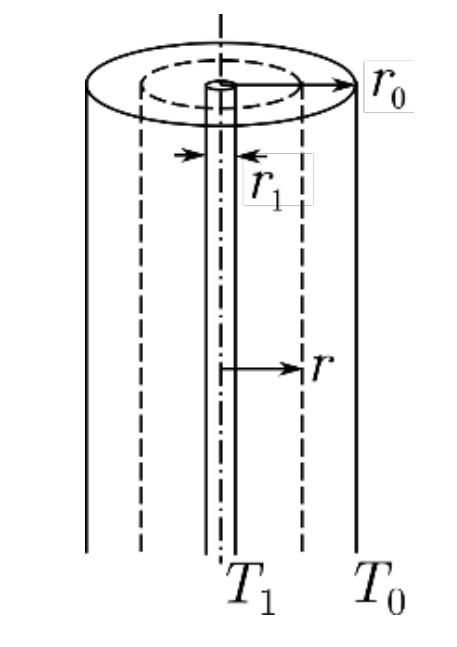
\includegraphics[scale=0.22]{picks/2_2_3_scheme1.jpg} \\
        \textit{\textcolor[HTML]{000000}{Рис. 1. Геометрия \\ задачи}}
    \end{center}
\end{minipage}

\formula
{}
{transFourier}
{q = -k\frac{dT}{dr}}

\newpage

\formula
{В стационарном состоянии полный поток тепла через любую цилиндрическую поверхность радиуса r площадью  \mth{S = 2\pi rL} должен быть одинаков и равен \mth{Q = qS}:}
{formQ}
{Q = -2\pi rL\cdot k\frac{dT}{dr} = const}

Если перепад температуры  \mth{\Delta T = T_1 - T_0} между нитью и стенками цилиндра мал \mth{(\Delta T << T_0),} то в (\ref{formQ}) можно пренебречь изменением теплопроводности от температуры в пределах системы, положив \mth{\chi \approx \chi(T_0)}. Тогда разделяя переменные в (\ref{formQ}) и интегрируя от радиуса нити до радиуса колбы получим:

\formula
{}
{finalQ}
{Q = \frac{2\pi L}{ln\frac{r_0}{r_1}} k\cdot \Delta T}

\vspace{1cm}

\begin{center}
    {\bf\Large
    Схема установки:}
    
    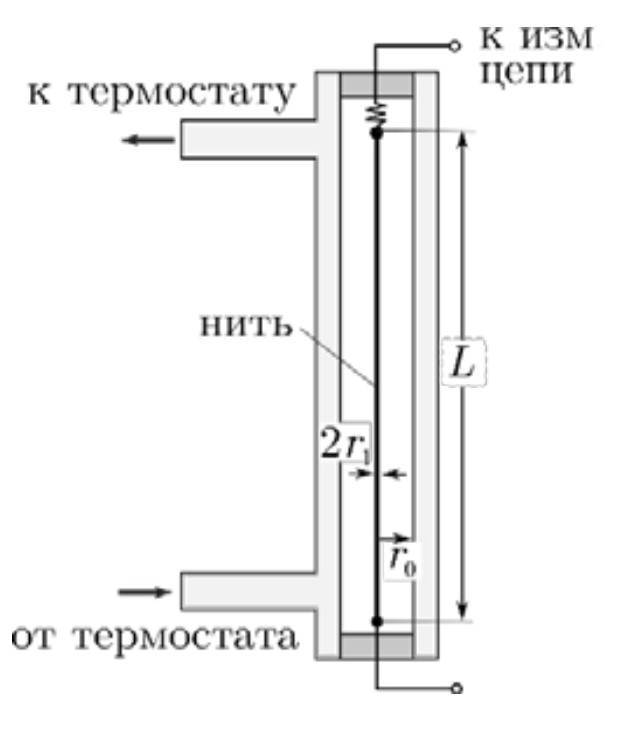
\includegraphics[scale=0.5]{picks/2_2_3_scheme2.jpg} \\
    \textit{\textcolor[HTML]{000000}{Рис. 2. Схема установки}}
    
\end{center}

\newpage
    	%!!! Experiment results and data here !!!%

\section{\Large Ход работы}

\begin{center}
    {\Large\bf Подготовка к эксперименту}
\end{center}

\subsection{Предварительные расчеты}
\hspace{1cm}Провел предварительные расчёты параметров опыта. Приняв максимально допустимый перегрев нити относительно термостата равным \mth{\Delta t_{max} = 10^\circ C}, оценил максимальную мощность нагрева \mth{Q_{max}[\text{мВт}],} которую следует подавать на нить. Для этой оценки принял коэффициент теплопроводности воздуха \mth{k \,\, \mathtt{\sim} \,\, 25 \frac{\text{мВт}}{\text{м}\cdot K}} \\

\noindent\hspace{1cm}Зная приблеженное значение сопростивления нити R, определил  соответствующие значения максимального тока \mth{I_{max}} и максимального напряжения \mth{U_{max}} \\

\noindent\hspace{1cm}{\bfПолученные значения:} \\[0.2cm]

\noindent\mth{Q_{max} = 102,9 \,\text{мВт}}\\

\noindent\mth{R = 13,0 \,\text{Ом}}\\

\noindent\mth{I_{max} = 89,0 \,\text{мА}}\\

\noindent\mth{U_{max} = 1,16 \,\text{В}}\\

\subsection{Подготовил эксперементальную установку к работе:}

\hspace{2cm}\begin{minipage}[t]{15cm}
\begin{itemize}
    \item Проверил, что измерительная схема собрана правильно;
    
    \item На магазине сопротивлений (или на реостате) установил максимальное сопростивление \mth{R\ruB{м}} ((чтобы ток в цепи при её замыкании был минимален);
    
    \item Включил вольтметр и амперметр и настроил режимы их работы (по техническому описанию к установке);

    \item Включил источник питания; проверил, что он работает в режиме источника напряжения, и что напряжение на нём не превышает максимально допустимое (указано на установке);
    
    \item Включил термостат и убедился, что вода в нём находится при комнатной температуре (измеренной по комнатному термометру).
    
\end{itemize}
\end{minipage}

\newpage

\begin{center}
    {\Large\bf Проведение измерений}
\end{center}

\subsection{Измерение зависимости R(Q)}
Провел серии экспериментов при разных температурах. \mth{U\ruB{э}} - Напряжение на эталонном сопротивлении; \mth{U\ruB{н}} - Напряжение на нити; R - Расчетное сопротивление нити; Q - Расчетная мощность на нити. Результаты представлены в таблице 1:

    \begin{table}[h!]
    	\begin{center}
    		\caption*{\color[HTML]{000000}Таблица 1: Измерение зависимости R(Q)}
    		\begin{tabular}{||P{3cm}|P{1.3cm}|P{1.3cm}|P{1.3cm}|P{1.3cm}|P{1.3cm}|P{1.3cm}|P{1.3cm}|P{1.3cm}||}
    	
    			\hline
    			\multicolumn{9}{||c||}{t = \mth{25,4^\circ} C} \\
    			\hline
    			
    			U\mth{\ruB{э}}, мВ & 50,0 & 75,0 & 100,0 & 200,0 & 350,0 & 500,0 & 700,0 & 850,0 \\
    			\hline
    			U\mth{\ruB{н}}, мВ & 62,5 & 93,8 & 124,9 & 249,8 & 438,9 & 628,8 & 885,4 & 1081,7 \\
    			\hline
    			R, Ом   & 12,56 & 12,51 & 12,49 & 12,49 & 12,54 & 12,58 & 12,66 & 12,73 \\
    			\hline
    			Q, мВт & 0,31 & 0,70 & 1,25 & 5,00 & 15,36 & 31,44 & 62,01 & 91,94\\

                \hline
    			\hline
    			\multicolumn{9}{||c||}{t = \mth{30,2^\circ} C} \\
    			\hline
    			
    			U\mth{\ruB{э}}, мВ  & 50,0 & 75,0 & 100,0 & 200,0 & 350,0 & 500,0 & 700,0 & 850,0 \\
    			\hline
    			U\mth{\ruB{н}}, мВ  & 63,7 & 95,7 & 127,6 & 255,5 & 447,8 & 642,1 & 903,2 & 1104,0 \\
    			\hline
    			R, Ом   & 12,74 & 12,76 & 12,76 & 12,78 & 12,79 & 12,84 & 12,90 & 12,99 \\
    			\hline
    			Q, мВт & 0,32 & 0,72 & 1,28 & 5,11 & 15,67 & 32,10 & 63,22 & 93,84 \\

    			\hline
    			\hline
    			\multicolumn{9}{||c||}{t = \mth{40,1^\circ} C} \\
    			\hline
    			
    			U\mth{\ruB{э}}, мВ  & 50,0 & 75,0 & 100,0 & 200,0 & 350,0 & 500,0 & 700,0 & 840,0 \\
    			\hline
    			U\mth{\ruB{н}}, мВ  & 65,6 & 98,4 & 131,1 & 262,5 & 460,2 & 659,5 & 928,2 & 1120,1 \\
    			\hline
    			R, Ом   & 13,12 & 13,12 & 13,11 & 13,13 & 13,15 & 13,19 & 13,26 & 13,33 \\
    			\hline
    			Q, мВт & 0,33  & 0,74  & 1,31  & 5,25 & 16,11 & 32,98 & 64,97 & 94,09 \\
    			
    			
                \hline
    			\hline
    			\multicolumn{9}{||c||}{t = \mth{50,4^\circ} C} \\
    			\hline
    			
    			U\mth{\ruB{э}}, мВ  & 50,0 & 75,0  & 100,0 & 200,0 & 350,0 & 500,0 & 700,0 & 800,0 \\
    			\hline
    			U\mth{\ruB{н}}, мВ  & 67,5 & 101,2 & 135,0 & 270,4 & 474,0 & 679,1 & 956,3 & 1096,2 \\
    			\hline
    			R, Ом   & 13,50 & 13,49 & 13,50 & 13,52 & 13,55 & 13,58 & 13,66 & 13,70 \\
    			\hline
    			Q, мВт & 0,34  & 0,76  & 1,35  & 5,41 & 16,60 & 33,95 & 66,94 & 87,70 \\
    
                \hline			
    			\hline
    			\multicolumn{9}{||c||}{t = \mth{60,4^\circ} C} \\
    			\hline
    			
    			U\mth{\ruB{э}}, мВ  & 50,0 & 75,0  & 100,0 & 200,0 & 350,0 & 500,0 & 700,0 & 800,0 \\
    			\hline
    			U\mth{\ruB{н}}, мВ  & 69,3 & 104,0 & 138,6 & 277,4 & 486,4 & 697,0 & 981,0 & 1125,0 \\
    			\hline
    			R, Ом   & 13,86 & 13,87 & 13,86 & 13,87 & 13,90 & 13,94 & 14,01 & 14,06 \\
    			\hline
    			Q, мВт & 0,35  & 0,78  & 1,39  & 5,55 & 17,02 & 34,85 & 68,67 & 90,00 \\
    			
                \hline
    		\end{tabular}
    	\end{center}
    \end{table}
    
\newpage
    	
%!!! Calculations result and graphs here !!!%

\subsection{График зависимостей R(Q)}

Построил график для зависимостей R(Q) при разных температурах. \\График представлен на Рис. 3. \\

\begin{center}
    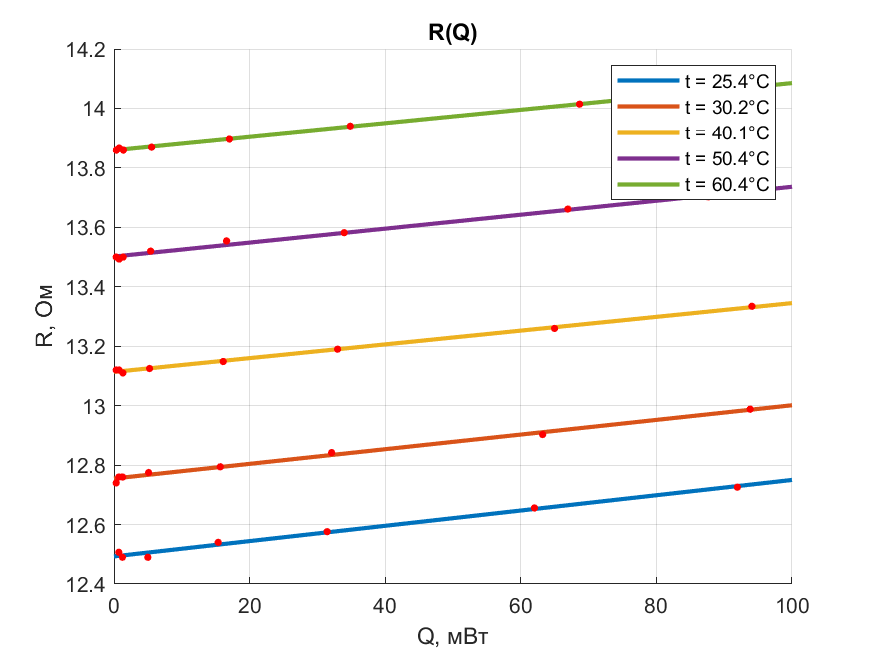
\includegraphics[scale = 1.3]{picks/223_R(Q).png} \\
    \textit{\textcolor[HTML]{000000}{Рис. 3. R(Q) для разных температур}}
\end{center}

\vspace{0.5cm}

    \begin{table}[h!]
    	\begin{center}
    		\caption*{\color[HTML]{000000}Таблица 2: Значения угловых к-тов \mth{\frac{dR}{dQ}} и значения R(0) для графика R(Q)}
    		\begin{tabular}{|P{3cm}|P{1.3cm}|P{1.3cm}|P{1.3cm}|P{1.3cm}|P{1.3cm}|}
    		\hline

                \mth{t, ^\circ C}    		& 25,4  & 30,2  & 40,1  & 50,4  & 60,4 \\  
    		    \hline
    		    R(0), Ом                    & 12,49 & 12,75 & 13,11 & 13,50 & 13,86 \\
    		    \hline
                \mth{\frac{dR}{dQ}, \frac{\text{Ом}}{\text{Вт}}}  & 2,57 & 2,46 & 2,31 & 2,34 & 2,25 \\


            \hline    		
    		\end{tabular}
    	\end{center}
    \end{table}

\newpage

\subsection{График зависимости R(t)}

Построил график для зависимости R(t). \\График представлен на Рис. 4. \\

\begin{center}
    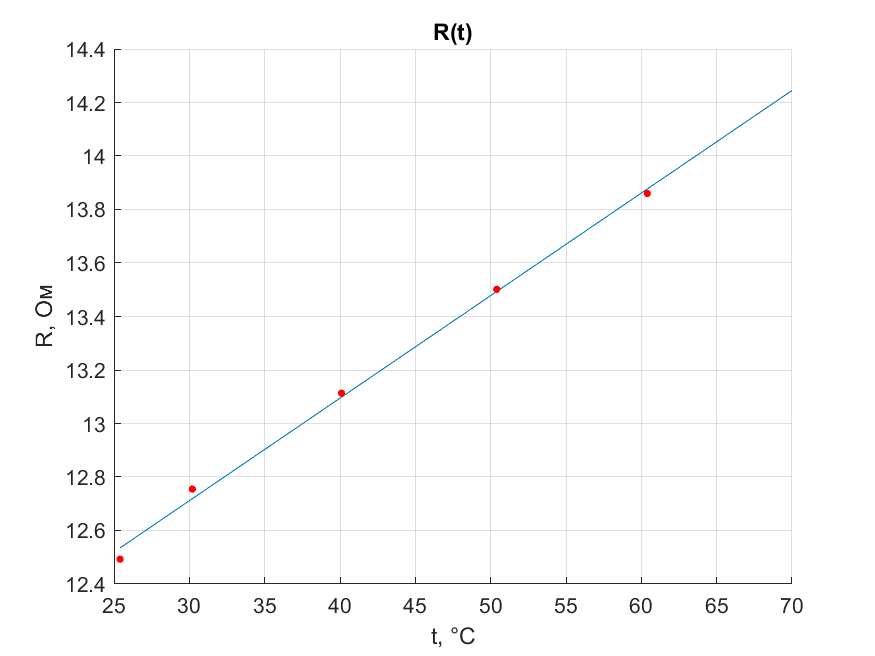
\includegraphics[scale = 1.3]{picks/223_R(T).png} \\
    \textit{\textcolor[HTML]{000000}{Рис. 4. R(t)}}
\end{center} 

\vspace{0.5cm}

Значение углового к-та для данного графика \mth{\frac{dR}{dT} = 3,83\cdot10^{-2} \frac{\text{Ом}}{K}}

\newpage

\subsection{Вычисление к-та теплопроводности при разных температурах термостата }

Из формулы (\ref{finalQ}) получил следующую формулу для расчета к: \\[0.2cm] 

\noindent\mth{k = \frac{\frac{dQ}{dR}\frac{dR}{dT}\,\cdot\, ln\frac{r_0}{r_1}}{2\pi L}} \\[0.2cm]

\noindent\mth{T_0} - Температура термостата; k - Значение теплопроводности. Результаты расчетов представлены в Таблице 3:

\begin{table}[h!]
    \begin{center}
        \caption*{\color[HTML]{000000}Таблица 3: к (T\mth{_0})}
        \begin{tabular}{|P{3cm}|P{1.3cm}|P{1.3cm}|P{1.3cm}|P{1.3cm}|P{1.3cm}|}
        \hline

            \mth{T_0, ^\circ C}    		         & 25,4  & 30,2  & 40,1  & 50,4  & 60,4 \\  
            \hline
            \mth{k, \frac{\text{Ом}}{\text{м}K} \cdot 10^{-2}} & 2,67 & 2,78 & 2,96 & 2,92 & 3,04 \\

        \hline    		
        \end{tabular}
    \end{center}
\end{table}

\subsection{График к(T)}

Пользуясь значениями из предыдущего пункта построил график к(T).\linebreak График представлен на рис. 5. \\

\begin{center}
    \includegraphics[scale = 1.0]{picks/223_k(T).png} \\
    \textit{\textcolor[HTML]{000000}{Рис. 5. k(t)}}
\end{center} 

\end{document}
